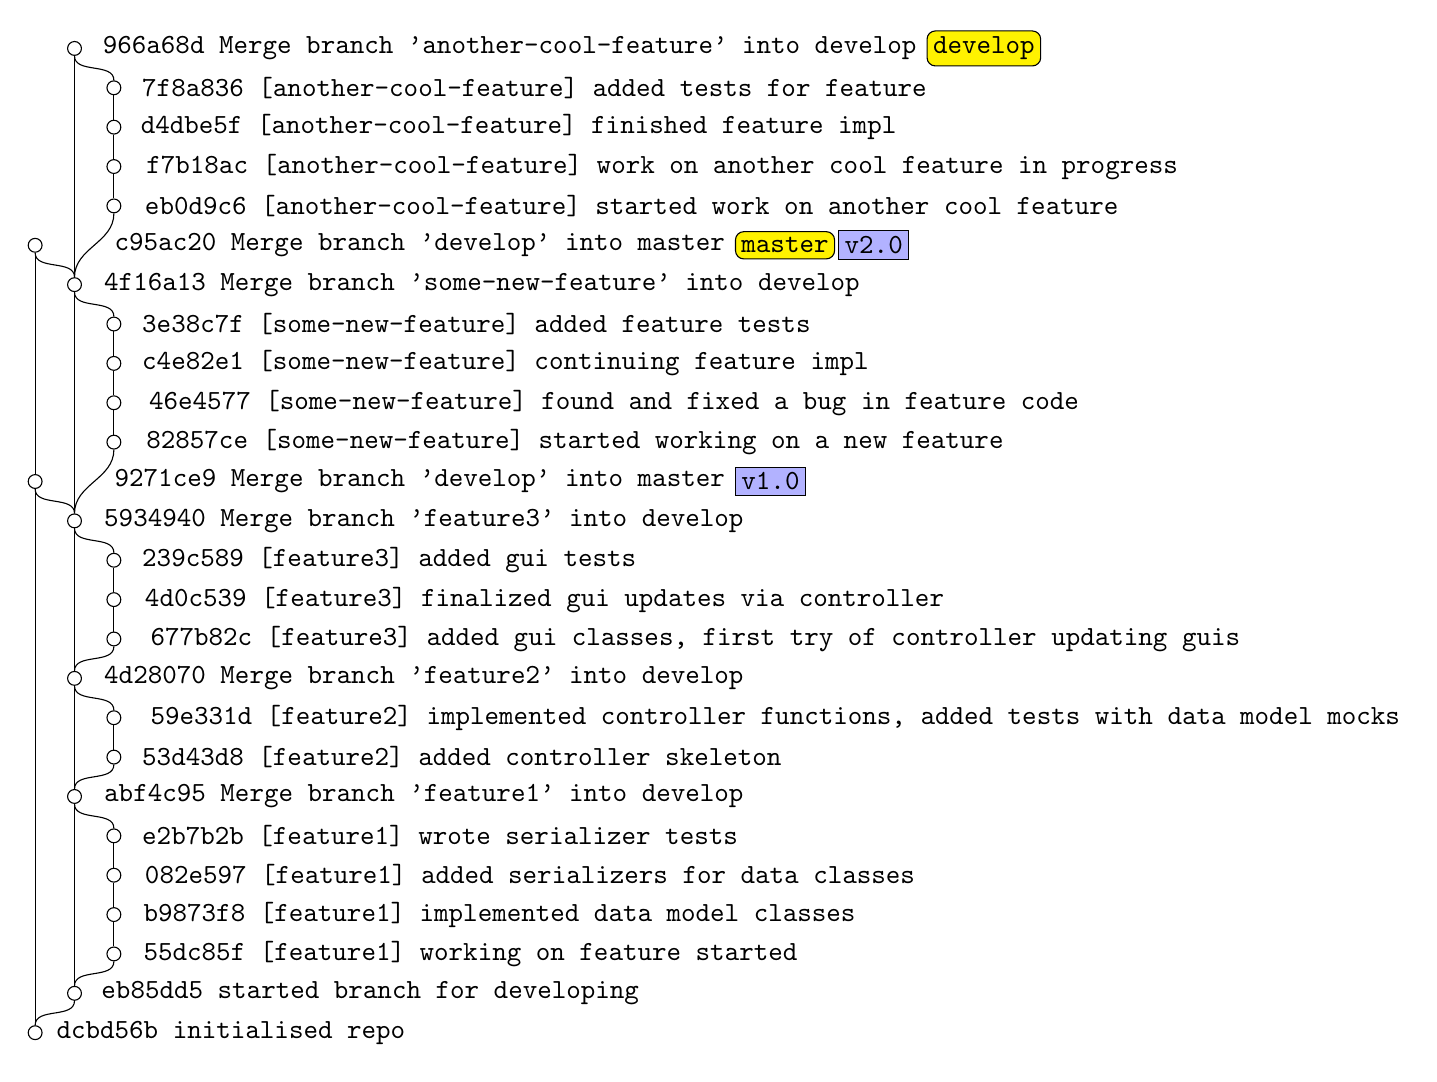
\begin{tikzpicture}

\tikzstyle{commit}=[draw,circle,fill=white,inner sep=0pt,minimum size=5pt]
\tikzstyle{clabel}=[right,outer sep=1em]
\tikzstyle{every path}=[draw]
\tikzstyle{branch}=[draw,rectangle,rounded corners=3,fill=yellow,inner sep=.5ex,minimum width=2ex, minimum height=2ex]
\tikzstyle{tag}=[draw,rectangle,fill=blue!30,inner sep=.5ex,minimum width=2ex, minimum height=2ex]

\node[commit] (966a68d) at (0.0,0) {};
\node[right,xshift=4.0] (label_966a68d) at (966a68d.east) {\verb!966a68d Merge branch 'another-cool-feature' into develop!};
\node[commit] (7f8a836) at (0.5,-0.5) {};
\node[right,xshift=4.0] (label_7f8a836) at (7f8a836.east) {\verb!7f8a836 [another-cool-feature] added tests for feature!};
\path (7f8a836) to[out=90,in=-90] (966a68d);
\node[commit] (d4dbe5f) at (0.5,-1.0) {};
\node[right,xshift=3.5] (label_d4dbe5f) at (d4dbe5f.east) {\verb!d4dbe5f [another-cool-feature] finished feature impl!};
\path (d4dbe5f) to[out=90,in=-90] (7f8a836);
\node[commit] (f7b18ac) at (0.5,-1.5) {};
\node[right,xshift=5.5] (label_f7b18ac) at (f7b18ac.east) {\verb!f7b18ac [another-cool-feature] work on another cool feature in progress!};
\path (f7b18ac) to[out=90,in=-90] (d4dbe5f);
\node[commit] (eb0d9c6) at (0.5,-2.0) {};
\node[right,xshift=5.0] (label_eb0d9c6) at (eb0d9c6.east) {\verb!eb0d9c6 [another-cool-feature] started work on another cool feature!};
\path (eb0d9c6) to[out=90,in=-90] (f7b18ac);
\node[commit] (c95ac20) at (-0.5,-2.5) {};
\node[right,xshift=22.5] (label_c95ac20) at (c95ac20.east) {\verb!c95ac20 Merge branch 'develop' into master!};
\node[commit] (4f16a13) at (0.0,-3.0) {};
\node[right,xshift=4.5] (label_4f16a13) at (4f16a13.east) {\verb!4f16a13 Merge branch 'some-new-feature' into develop!};
\path (4f16a13) to[out=90,in=-90] (966a68d);
\path (4f16a13) to[out=90,in=-90] (eb0d9c6);
\path (4f16a13) to[out=90,in=-90] (c95ac20);
\node[commit] (3e38c7f) at (0.5,-3.5) {};
\node[right,xshift=4.0] (label_3e38c7f) at (3e38c7f.east) {\verb!3e38c7f [some-new-feature] added feature tests!};
\path (3e38c7f) to[out=90,in=-90] (4f16a13);
\node[commit] (c4e82e1) at (0.5,-4.0) {};
\node[right,xshift=4.0] (label_c4e82e1) at (c4e82e1.east) {\verb!c4e82e1 [some-new-feature] continuing feature impl!};
\path (c4e82e1) to[out=90,in=-90] (3e38c7f);
\node[commit] (46e4577) at (0.5,-4.5) {};
\node[right,xshift=6.5] (label_46e4577) at (46e4577.east) {\verb!46e4577 [some-new-feature] found and fixed a bug in feature code!};
\path (46e4577) to[out=90,in=-90] (c4e82e1);
\node[commit] (82857ce) at (0.5,-5.0) {};
\node[right,xshift=5.5] (label_82857ce) at (82857ce.east) {\verb!82857ce [some-new-feature] started working on a new feature!};
\path (82857ce) to[out=90,in=-90] (46e4577);
\node[commit] (9271ce9) at (-0.5,-5.5) {};
\node[right,xshift=22.5] (label_9271ce9) at (9271ce9.east) {\verb!9271ce9 Merge branch 'develop' into master!};
\path (9271ce9) to[out=90,in=-90] (c95ac20);
\node[commit] (5934940) at (0.0,-6.0) {};
\node[right,xshift=4.5] (label_5934940) at (5934940.east) {\verb!5934940 Merge branch 'feature3' into develop!};
\path (5934940) to[out=90,in=-90] (4f16a13);
\path (5934940) to[out=90,in=-90] (82857ce);
\path (5934940) to[out=90,in=-90] (9271ce9);
\node[commit] (239c589) at (0.5,-6.5) {};
\node[right,xshift=4.0] (label_239c589) at (239c589.east) {\verb!239c589 [feature3] added gui tests!};
\path (239c589) to[out=90,in=-90] (5934940);
\node[commit] (4d0c539) at (0.5,-7.0) {};
\node[right,xshift=5.0] (label_4d0c539) at (4d0c539.east) {\verb!4d0c539 [feature3] finalized gui updates via controller!};
\path (4d0c539) to[out=90,in=-90] (239c589);
\node[commit] (677b82c) at (0.5,-7.5) {};
\node[right,xshift=7.0] (label_677b82c) at (677b82c.east) {\verb!677b82c [feature3] added gui classes, first try of controller updating guis!};
\path (677b82c) to[out=90,in=-90] (4d0c539);
\node[commit] (4d28070) at (0.0,-8.0) {};
\node[right,xshift=4.5] (label_4d28070) at (4d28070.east) {\verb!4d28070 Merge branch 'feature2' into develop!};
\path (4d28070) to[out=90,in=-90] (5934940);
\path (4d28070) to[out=90,in=-90] (677b82c);
\node[commit] (59e331d) at (0.5,-8.5) {};
\node[right,xshift=7.0] (label_59e331d) at (59e331d.east) {\verb!59e331d [feature2] implemented controller functions, added tests with data model mocks!};
\path (59e331d) to[out=90,in=-90] (4d28070);
\node[commit] (53d43d8) at (0.5,-9.0) {};
\node[right,xshift=4.0] (label_53d43d8) at (53d43d8.east) {\verb!53d43d8 [feature2] added controller skeleton!};
\path (53d43d8) to[out=90,in=-90] (59e331d);
\node[commit] (abf4c95) at (0.0,-9.5) {};
\node[right,xshift=4.5] (label_abf4c95) at (abf4c95.east) {\verb!abf4c95 Merge branch 'feature1' into develop!};
\path (abf4c95) to[out=90,in=-90] (4d28070);
\path (abf4c95) to[out=90,in=-90] (53d43d8);
\node[commit] (e2b7b2b) at (0.5,-10.0) {};
\node[right,xshift=4.0] (label_e2b7b2b) at (e2b7b2b.east) {\verb!e2b7b2b [feature1] wrote serializer tests!};
\path (e2b7b2b) to[out=90,in=-90] (abf4c95);
\node[commit] (082e597) at (0.5,-10.5) {};
\node[right,xshift=5.0] (label_082e597) at (082e597.east) {\verb!082e597 [feature1] added serializers for data classes!};
\path (082e597) to[out=90,in=-90] (e2b7b2b);
\node[commit] (b9873f8) at (0.5,-11.0) {};
\node[right,xshift=4.5] (label_b9873f8) at (b9873f8.east) {\verb!b9873f8 [feature1] implemented data model classes!};
\path (b9873f8) to[out=90,in=-90] (082e597);
\node[commit] (55dc85f) at (0.5,-11.5) {};
\node[right,xshift=4.5] (label_55dc85f) at (55dc85f.east) {\verb!55dc85f [feature1] working on feature started!};
\path (55dc85f) to[out=90,in=-90] (b9873f8);
\node[commit] (eb85dd5) at (0.0,-12.0) {};
\node[right,xshift=3.5] (label_eb85dd5) at (eb85dd5.east) {\verb!eb85dd5 started branch for developing!};
\path (eb85dd5) to[out=90,in=-90] (abf4c95);
\path (eb85dd5) to[out=90,in=-90] (55dc85f);
\node[commit] (dcbd56b) at (-0.5,-12.5) {};
\node[right,xshift=1.5] (label_dcbd56b) at (dcbd56b.east) {\verb!dcbd56b initialised repo!};
\path (dcbd56b) to[out=90,in=-90] (9271ce9);
\path (dcbd56b) to[out=90,in=-90] (eb85dd5);
\node[branch,right,xshift=.1] (develop) at (label_966a68d.east) {\verb!develop!};
\node[branch,right,xshift=.1] (master) at (label_c95ac20.east) {\verb!master!};
\node[tag,right,xshift=.1] (label_tag_v1.0) at (label_9271ce9.east) {\verb!v1.0!};
\node[tag,right,xshift=1.1] (label_tag_v2.0) at (master.east) {\verb!v2.0!};
\end{tikzpicture}